Two-dimensional images mapped to three-dimensional objects, referred to as \textit{textures}, have long been used to efficiently add pre-calculated details to a 3D scene in computer graphics. In the past decade however, procedural textures have gained an increasing amount of traction as a serious contender to the traditional bitmap texture. The procedural approach presents a new way of generating textures mathematically with a high level of editability, arbitrary levels of detail, compactness and seamless transition between object faces, see Figure \ref{fig:BitmapVsProcedural}. With programs such as Blender or Substances Designer growing in popularity and being adopted by industry professionals, tools for creating procedural texture models using node graph editors are now more accessible than ever \cite{blenderfoundation_2020_blenderorg, a2020_substance}. 

Despite its very appealing advantages, procedural textures remain an advanced alternative to traditional texturing methods in offline rendering for mainly one reason alone; they are difficult to design in order to achieve desired results. While modern tools present users with a node editor that abstracts away the underlying functions, figuring out how to compose nodes and what values to assign the sometimes hundreds of parameters in order to achieve desired results, is very convoluted and time-consuming. Recent advances in texture synthesis using neural networks, e.g. \textit{TileGAN}, presents an exemplar based alternative that can generate higher quality versions of user example textures, although not solving the problems with seams and lack of compactness of traditional textures \cite{frhstck_2019_tilegan}. Still, texture synthesis is an example of an \textit{inverse} modeling process that is easy to operate for a novel user, especially as a plethora of bitmap images are already available for free on the web which can serve as a target for such an inverse problem. 

This thesis focuses on a problem within \textit{inverse procedural texture modeling}, a research field that aims to inverse the rendering process and estimate parameters of procedural texture models such that the rendered result matches an input image. However, due to the complexity of most modern render engines built without this functionality in mind, the relationship between procedural model parameters is non-linear and near impossible to differentiate. Additionally, developing a suitable loss function that can measure image similarity is a non-trivial task, due to the discrepancy between the way computers and humans perceive images.

\begin{figure}
    \centering
    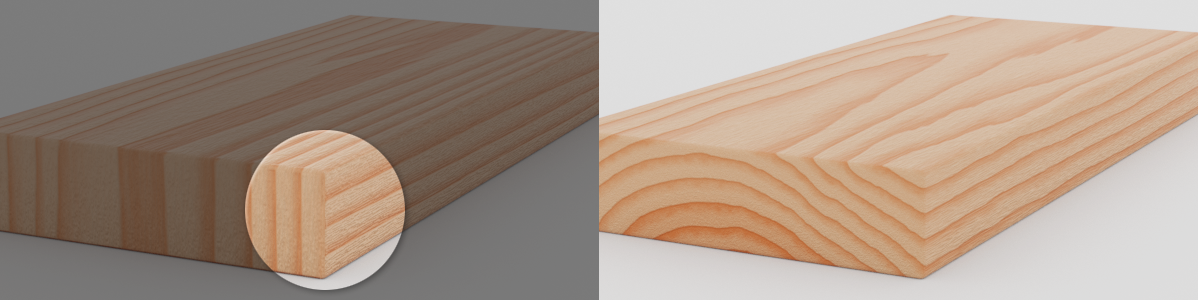
\includegraphics[width=\textwidth]{img/background/PlaneOrNotAPlane.png}
    \caption{Left$:$ Using a bitmap texture can result in visible seams between object faces as it is inherently difficult to naturally map a 2D texture onto a 3D object. Right$:$ A similar texture rendered with a procedural model. As procedural textures are functions of an object's 3D coordinates, a seamless result is achieved \cite{_comparison}.}
    \label{fig:BitmapVsProcedural}
\end{figure}

A few fully differentiable rendering engines have already been developed, such as \textit{OpenDR} or \textit{PyTorch3D}, but neither have direct support for procedural textures \cite{loper_2014_opendr, facebookresearch_2020_facebookresearchpytorch3d}. Recently Guo et. al published a paper detailing a framework for procedural parameter estimation using Bayesian inference \cite{guo_2019_a}. Their results are promising and the contribution of suitable loss functions serve as an inspiration for this thesis. However, their framework did not allow the user to compose their own procedural textures and only tested their algorithm on hard-coded procedural models. Intending to fill a gap in the field of inverse procedural texture modeling, we present DiPTeR, a Differentiable Procedural Texture Renderer that allows users to dynamically build fully differentiable procedural textures and automatically estimate its parameters using a target image. 

This project was initially conducted in Japan at the University of Tokyo as part of the HCI for machine learning focused group \textit{CREST}, led by Takeo Igarashi \cite{jstcrest_2020_jst}. In April 2020 the threat of the COVID-19 crisis forced the university to close, and we had to continue the project in Lund, Sweden unfortunately without access to Lund University's premises or equipment.

\section{Goal}

To alleviate the difficulties of creating complex procedural texture models by hand, our goal is to develop a \textit{Differentiable Procedural Texture Renderer} or DiPTeR, which can render procedural textures in OpenGL but also include a fully differentiable back-end renderer that mimics the rendering process of OpenGL. The back-end renderer should be written in a framework that allows for automatic differentiation, enabling us to create procedural functions and rendering procedures of arbitrary complexity while retaining differentiability. The framework should include a node editor, much like Blender and Substance Designer, that lets users easily build procedural texture models and observe their rendered results in real time. A user should also be able to present a target bitmap texture, and let the system automatically estimate the optimal parameter values of their procedural texture model. Automatically constructing the model itself is outside the scope of this project, and is an entirely different problem. Measuring the similarity between rendered texture and target texture is accomplished by means of loss functions, and the framework should allow the user to easily select and implement their own loss functions. While the framework is intended to be operated through a graphical interface developed by us, it should be possible to run the entire texture matching algorithm through a non-graphical user interface.

Through evaluation of our system, we would like to answer the following research questions: Is it possible to build a differentiable rendering system in PyTorch? Is it efficient enough to render in real time? Is it possible to mimic the intricacies of procedural texturing of OpenGL in PyTorch, including the use of noise? Can we achieve an acceptable parameter estimation for a complex procedural texture on a timescale of minutes? Can we find a loss function that performs well for many different types of procedural textures?

\section{Methodology}

This project was initialized by conducting a general literature review where we researched current and past methods of inverse rendering, specifically pertaining to procedural textures. Most papers pursued a neural network based solution which inspired our initial research plan to train a GAN on a dataset of procedurally rendered textures in order to perform regression on the procedural model parameters.

During the first seven weeks in Tokyo we developed an add-on for Blender to automatically render datasets to train on, as well as conducting some testing of our initial solution. Eventually we realized that this approach does not perform well on complex procedural textures and is not flexible enough. We then entered our second literature study phase and designed a new solution relying on explicit inverse rendering by using a differentiable renderer.

Our main development phase was then started and our solution implemented in Python, which was chosen for its excellent support for machine learning as well as fast and simple development. The implementation consists of three main parts, the differentiable renderer including shaders and parameter estimation implemented using the machine learning library PyTorch, the non-differentiable OpenGL rendering integrated in Python by the package Glumpy and lastly a graphical user interface implemented using PyQt5 \cite{paszke_2019_pytorch, rougier_2011_glumpy, riverbankcomputing_2020_what}.

Finally, our system was evaluated by designing three test shader models of increasing complexity and running parameter estimation on them for all combinations of optimizers and loss functions that we support, measuring the loss value at each iteration. Furthermore, rendering performance of our back-end render engine was evaluated as well as the time required to complete an iteration of gradient descent for each loss function.

\section{Contributions}

In this thesis we outline a novel approach to the under-researched problem of inverse procedural texture modeling by applying reliable techniques such as stochastic gradient descent. Specifically, our principal contributions are:

\begin{list}{$\diamond$}{}
    \item Implementing a fully differentiable, dynamic procedural texture renderer. Procedural textures can be dynamically created during run-time and rendered in real-time while maintaining differentiability.
    \item Pairing this differentiable renderer with OpenGL, a popular and modern computer graphics API, in such a way that users do not have to be aware that two systems are used in tandem. This allows for fast and familiar forward rendering in OpenGL as well as parameter estimation using our differentiable renderer, therefore enabling both rendering system to be exported to other projects separately.
    \item Using proven techniques for optimization such as stochastic gradient descent for procedural texture parameter estimation. To the best of our knowledge this has not been done before. 
    \item Developing a graphical user interface, including a node editor, enabling users to build composite procedural texture models.
    \item Developing a GLSL code parser framework to enable GLSL shader composition and compilation at run-time as well as code reuse through a custom preprocessor directive.
    \item Evaluating a number of different loss functions and optimizers for parameter estimation.
\end{list}

\section{Related Work}
This thesis primarily covers two topics; Inverse Rendering and Procedural Textures. Neither subject is new and both are well researched, but few papers attempt to combine the two. Many approaches to inverse rendering use neural networks, with good results for their somewhat narrow use cases. This thesis was born from inspiration of this method, but it was soon discovered that it is not a viable solution for our use case, where we allow users to freely modify and compose procedural textures, resulting in near endless pattern combinations. Training a neural network to perform well on such data would require an immense dataset to train on, as well as an extremely complex model. Instead, we chose a differentiable rendering approach using gradient descent to estimate procedural texture parameters, which to the best of our knowledge, has not been done before. This section analyzes a number of papers and frameworks whose solutions have directly affected this thesis.

\subsection{Inverse Procedural Texture Modeling}

A relatively low amount of research has been conducted within \textit{inverse procedural texture modeling}, a narrow subfield of computer science, which has nonetheless produced two recent papers that lay the foundation for this thesis. In 2019, Hu et. al. published \textit{A Novel Framework For Inverse Procedural Texture Modeling} in which they describe a framework for procedural texture model acquisition as well as parameter estimation for said model \cite{hu_2019_a}. A K-means algorithm is used to find the most suitable procedural texture model among a library of predefined models for a user's input texture. Each procedural texture has an associated Convolutional Neural Network model, used to solve the regression problem of finding an optimal parameter set to the procedural texture so that it renders an image similar to the user's input image. This approach is unfortunately not very flexible, as the procedural textures have to be predefined and training a neural network on each texture requires a considerable amount of effort and time. Using CNNs for regression also proved difficult for complex procedural texture models, and so neural networks were abandoned for this thesis altogether. 

A much different approach was formulated in the work by Guo et. al. in 2019, where their solution involves Bayesian inference and sampling of the space of plausible parameters to find an optimal parameter set for a chosen procedural texture \cite{guo_2019_a}. Similar to their work, we also implemented a solution in a differentiable framework, however, our system does not require any sampling techniques. Furthermore, they contribute by developing smart loss functions that do not depend on textures being pixel-wise aligned, some of which have been implemented in this thesis. Finally, unlike us they do not provide an interface to create procedural textures, and only offer hard-coded procedural textures.

\subsection{Differentiable Rendering}

An important foundation that allows our approach to work is the concept of differentiable rendering, that is, the ability to differentiate the entire rendering process, and thus obtain gradients for it. A few notable examples of this have been an inspiration when we developed our own differentiable renderer. Perhaps most notable is the very recently released PyTorch3D, a rendering framework developed by the team behind \textit{PyTorch} which was in fact used to implement our differentiable renderer \cite{facebookresearch_2020_facebookresearchpytorch3d, paszke_2019_pytorch}. PyTorch3D was unfortunately released without our knowledge around the same time as this thesis was started and shares many concepts, although their approach is more general and lack any advanced procedural texturing support. Earlier approaches like the OpenDR framework is closely related to our project, but with a different focus \cite{loper_2014_opendr}. OpenDR is a framework where the entire forward rendering process is differentiable, enabling the user to automatically compute scene parameters such as vertex positions, camera parameters and vertex colors. Our solution does not focus on the 3D model or camera parameters, but on per-pixel procedural colors and not only per-vertex colors. As much of our algorithm relies on writing differentiable shaders, we must not fail to mention an attempt to do just that, directly implemented in the HLSL shader language \cite{guenter_2011_symbolic}. This project was led by Microsoft Research and although their use case was more aimed towards calculating efficient normals, tangents and derivatives of sub-routines, it remains an interesting idea that would have been too complex to implement in this thesis.

\section{Report Outline}

The next chapter explains some of the theoretical background needed to understand this thesis. At the end of the chapter in section \ref{sec:BackgroundInverseGraphics}, some other similar forms of inverse graphics and related works are explained. Next, chapter 3 outlines the method used in this project, explaining the different parts of \dipter{}, including the graphical interface, as well as putting the theory into context. Chapter 4 then explains some of the implementation details on how our PyTorch shaders mimic OpenGL shaders and some details on the OpenGL rendering pipeline. In chapter 5 we explain the test setup and evaluation of our parameter estimation method on a number of test shaders and discuss the results. Finally, we draw a brief conclusion on the rendering and parameter estimation capabilities of \dipter{}, as well as suggest what could be done in the future to further improve our method.


